\section{Conclusion}

\subsection{Project Overview}

The study of these five technologies makes it possible to establish a comparative framework based on the analysis of various performance parameters (\cite{rpe_book} p. 622). In accordance with the literature, the most relevant parameters to consider are thrust, which reflects the system’s responsiveness; specific impulse, which indicates efficiency; total propulsion duration; and the power required to generate a unit of thrust.


\begin{table}[H]
    \centering
    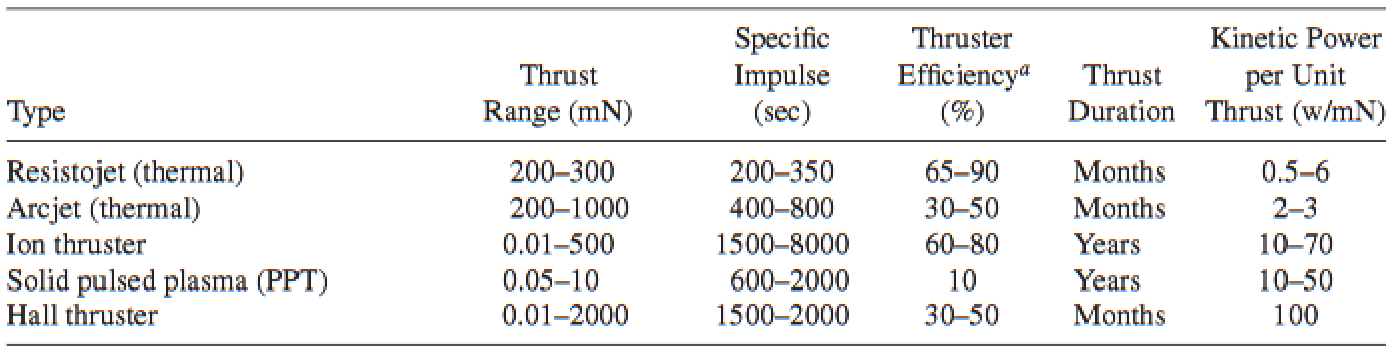
\includegraphics[width=1\linewidth]{figs/tab_recap_vf.png}
    \caption{Performance comparison of the different technologies}
    \label{tab:all_performances}
\end{table}

The selection of a given thruster ultimately depends on a trade-off between mission requirements and operational constraints. It can be observed that electrostatic and electromagnetic technologies generally achieve higher specific impulses—as is the case for ion thrusters—but produce lower thrust levels than electrothermal technologies.
\\

Ion propulsion and Hall-effect thrusters remain the most suitable options for applications that do not require high thrust levels, such as slow orbital maneuvers, station-keeping, or interplanetary and deep-space missions. They offer high specific impulse and superior efficiency compared to alternative electric propulsion technologies.

Conversely, electrothermal propulsion systems, while capable of delivering relatively higher thrust, are less attractive in terms of specific impulse, which remains only marginally higher than that of chemical propulsion systems. In addition, these technologies are subject to significant thermal losses, which further reduce their overall efficiency.

Pulsed Plasma Thrusters (PPT), although technologically advanced, remain limited in efficiency and thrust compared to other electric propulsion systems and is mainly used in small satellites due to their ease of implementation and robustness.
\\

Beyond efficiency considerations, practical factors must also be taken into account when evaluating these different thrusters, such as component erosion and system footprint. From this perspective, Hall-effect thrusters are among the most compact solutions. Ion thrusters and Pulsed Plasma Thrusters (PPT) are also less affected by erosion compared to other technologies (\cite{rpe_book} p. 624).

\subsection{Application Contexts of Electric Propulsion Systems}
This comparison highlights the respective advantages and limitations of each technology, providing a deeper understanding of why certain thrusters are more widely adopted in the industry depending on the application context.

Currently, ion thrusters are predominantly used for GEO satellites and deep-space exploration missions, while Hall-effect thrusters are more commonly employed for LEO and MEO satellites. Arcjet and resistojet technologies also retain relevance for specific applications requiring higher thrust while maintaining a specific impulse superior to that of chemical propulsion. In contrast, Pulsed Plasma Thruster (PPT) technology still faces significant limitations and remains relatively underutilized (\cite{rpe_book} p. 624).

\subsection{Most important things}

This study explores the technical details of electric propulsion and the operating principles of the technologies considered. However, from a broader perspective, it also highlights several general insights into electric propulsion systems. Based on this work, the following presents a non-exhaustive list of the key takeaways regarding electric propulsion:

\begin{enumerate}
	\item There are three main families of physical principles underlying electric propulsion technologies: electrostatic, electrothermal, and electromagnetic thrusters.
	\item Electric propulsion systems provide a higher specific impulse than chemical propulsion but generate significantly lower thrust levels.
	\item Due to their low thrust, electric propulsion systems are not suitable for launch or rapid maneuvers, as they require long operating times to produce significant velocity changes. However, electric propulsion is highly efficient for long-duration maneuvers and orbital corrections, owing to its high specific impulse.
	\item The low thrust levels enable precise control, making electric propulsion well suited for micropropulsion and fine attitude or trajectory adjustments.
	\item The most mature technologies are electrostatic thrusters, particularly ion and Hall-effect thrusters. Other systems, such as resistojets, arcjets, and pulsed plasma thrusters (PPT), still face significant challenges, including limited energy efficiency and electrode erosion.
	\item The primary limitation of electric propulsion is not the availability of propellant, but the available power. This power can be generated from solar energy or supplied by nuclear sources, the latter offering significantly higher energy density than chemical fuels.
\end{enumerate}

In conclusion, the propellant mass required over the lifetime of a spacecraft is significantly higher for chemical propulsion systems:

\begin{center}
\textit{“For NSSK the satellite might need an annual velocity increase of some 50 m/sec; this requires about 750 kg of chemical propellant for the entire period, which is more than one-quarter of the satellite mass. Using an electric propulsion system with a specific impulse of 2800 sec (about nine times higher than a chemical rocket), the propellant mass can be reduced to perhaps less than 100 kg” (\cite{rpe_book} p.625).}
\end{center}

In the context of space systems, every kilogram of mass represents an additional cost, and it is often more beneficial to allocate this mass budget to payload instruments rather than propellant. A quantitative example highlights this advantage:


\begin{center}
\textit{“With launch costs estimated at \$50,000 per kilogram delivered to GEO, this is a potential saving of \$22,500,000 per satellite” (\cite{rpe_book} p.625)}
\end{center}


Electric propulsion systems therefore offer significant practical and economic advantages, which explains their widespread adoption in the space industry today.

As space missions continue to evolve toward longer durations, higher efficiency, and reduced mass constraints, electric propulsion is expected to play an increasingly dominant role. Ongoing advancements in power systems, materials, and plasma physics will likely further enhance the performance and reliability of these technologies, reinforcing their importance in the future of space exploration.